\subsection{连续谱、预解边界值与 Robin 完备关系}

区间上的离散正交基在无限区域不再适用。预解边界值既恢复连续谱密度，也把边界束缚态与散射模态放到同一完备关系中。

前面的谱定理给出了自伴算子的统一表达，却没有要求谱必须由平方可积的本征函数构成。对于非紧空间，连续谱和边界散射必须直接通过预解算子处理。

在紧致球面上，正交球谐构成离散基；然而在无限伸展的空间里，典型自由粒子并没有平方可积的能量本征态。若把连续谱误写成离散求和，就会同时破坏态的归一化、Green 核和远场条件。一般空间的高频理论因此不能止于紧致截面的表示分解；还必须从谱测度本身理解连续谱和散射。

设 $A$ 是 Hilbert 空间 $\Hil$ 上的自伴算子。其谱 $\operatorname{spec}A$ 分为点谱与连续谱等部分：$Au=\lambda u$ 存在非零 $L^2$ 解时 $\lambda$ 是本征值；若存在归一化序列 $u_j\in\operatorname{Dom}A$，满足 $\|(A-\lambda)u_j\|\to0$，那么 $\lambda$ 属于谱，但并不保证存在 $L^2$ 本征向量。这样的序列称为 Weyl 序列，它可以将质量逐渐推向空间无穷远。

\begin{definition}[预解式与边界值]
对 $z\in\CC\setminus\operatorname{spec}A$，预解算子是
\begin{equation}\label{eq:ghs-r6-resolvent-definition}
R_A(z)=(A-z)^{-1}.
\end{equation}
当谱覆盖实轴的一部分时，$R_A(\lambda\pm\ii0)$ 一般不作为 $L^2\to L^2$ 的有界算子存在。若其极限在适当加权 Sobolev 空间之间成立，才可称为边界值预解算子。
\end{definition}

由 $R_A(z)(A-z)=I$ 可以直接推得预解恒等式
\begin{equation}\label{eq:ghs-r6-resolvent-identity}
R_A(z)-R_A(w)=(z-w)R_A(z)R_A(w).
\end{equation}
它说明不同复能量上的 Green 算子并非独立函数；而谱测度的密度可从实谱上下边界值的跃变提取。这一关系以后会把散射态的选择与辐射条件联系起来。

在 $\Hil=L^2(\RR,\dd x)$ 上取自伴算子 $A=-\partial_x^2$，定义域为 Sobolev 空间 $H^2(\RR)$。为求 $G_z(x,y)$，解
\[
(-\partial_x^2-z)G_z(x,y)=\delta(x-y).
\]
选 $k=\sqrt z$ 的分支满足 $\operatorname{Im}k>0$。源点两侧满足 $G''+k^2G=0$；为使远离源点时指数衰减，两侧只能分别选取 $\ee^{\ii k(x-y)}$ 或 $\ee^{-\ii k(x-y)}$。因此设
\[
G_z(x,y)=C\ee^{\ii k|x-y|}.
\]
为了消去微分后的 $\delta$ 以外的奇性，$G_z$ 在 $x=y$ 连续，而一阶导数跳跃必须满足
\[
-\bigl[\partial_xG_z(y^+,y)-\partial_xG_z(y^-,y)\bigr]=1.
\]
代入后得 $-2\ii kC=1$，故
\begin{equation}\label{eq:ghs-r6-line-resolvent}
R_A(z)(x,y)=\frac{\ii}{2\sqrt z}\ee^{\ii\sqrt z|x-y|},
\quad\operatorname{Im}\sqrt z>0.
\end{equation}
在 $z=-\kappa^2$、$\kappa>0$ 处，选择 $\sqrt z=\ii\kappa$ 后立即得到
\[
R_A(-\kappa^2)(x,y)=\frac{1}{2\kappa}\ee^{-\kappa|x-y|}.
\]
这个指数核在 $\kappa\to0$ 时没有有界的极限，这不是推导出了矛盾，而是因为自由 拉普拉斯算子 的谱从零开始，零能阈值没有谱隙。

\begin{theorem}[从预解跃变恢复自由谱密度]\label{thm:ghs-r6-stone-line}
对 $A=-\partial_x^2$ 的绝对连续谱，设 $\lambda=k^2>0$，则
\begin{equation}\label{eq:ghs-r6-free-spectral-density}
\frac{\dd\mathsf E_A(\lambda)}{\dd\lambda}(x,y)
=\frac{\cos(k(x-y))}{2\pi k}.
\end{equation}
\end{theorem}
\begin{proof}
沿实谱上下靠近时，$R_A(\lambda+\ii0)$ 使用外向波 $\ee^{\ii k|x-y|}$，而自伴性给
$R_A(\lambda-\ii0)(x,y)=\overline{R_A(\lambda+\ii0)(y,x)}$
$=-\ii\ee^{-\ii k|x-y|}/(2k)$。两者相减，
\[
R_A(\lambda+\ii0)-R_A(\lambda-\ii0)
=\frac{\ii}{k}\cos(k(x-y)).
\]
在弱分布意义下使用 Stone 公式
\[
\dd\mathsf E_A(\lambda)=\frac{1}{2\pi\ii}
(R_A(\lambda+\ii0)-R_A(\lambda-\ii0))\dd\lambda
\]
即得所写密度。检验归一化时以 $\dd\lambda=2k\dd k$ 换变量，
\[
\int_0^\infty\frac{\cos(k(x-y))}{2\pi k}\,2k\dd k
=\int_0^\infty\frac{\cos(k(x-y))}{\pi}\dd k=\delta(x-y)
\]
按 Fourier 分布恒等式成立。若遗漏 雅可比因子 $2k$，就无法恢复单位算子。
\end{proof}

在 $L^2(0,\infty)$ 上取同一个微分表达式 $-\partial_x^2$。若在 $x=0$ 施加 Dirichlet 边界条件，其 Green 核可以用镜像构造：
\begin{equation}\label{eq:ghs-r6-halfline-green}
R_D(-\kappa^2)(x,y)=\frac{1}{2\kappa}
\left[\ee^{-\kappa|x-y|}-\ee^{-\kappa(x+y)}\right].
\end{equation}
第二项专门负责在 $x=0$ 抵消第一项，它没有改变源点的导数跳跃。解析延拓并计算 Stone 跃变后得到
\begin{equation}\label{eq:ghs-r6-halfline-density}
\frac{\dd\mathsf E_D(\lambda)}{\dd\lambda}(x,y)
=\frac{\sin(kx)\sin(ky)}{\pi k},\qquad k=\sqrt\lambda>0.
\end{equation}
因此完备关系是
\[
\int_0^\infty\frac{2}{\pi}\sin(kx)\sin(ky)\dd k=\delta(x-y),
\]
恰是 Fourier 正弦变换。若改用 Neumann 条件，镜像项由负号改为正号，对应余弦变换。两种自伴实现都有连续谱 $[0,\infty)$，但谱核、边界模态和零能行为不同。

谱定理本身并不解决奇点附近允许什么边界数据的问题。在圆锥或球坐标中，径向约化会产生逆平方势；它的自伴定义域仍须由端点的可积解决定。

现在回到 $\RR^n\setminus\{0\}$。取标准单位球面上的球谐 $Y_{\ell a}$，满足 $-\Delta_{S^{n-1}}Y_{\ell a}=\ell(\ell+n-2)Y_{\ell a}$，并设
\[
\phi(r,\Omega)=f_\ell(r)Y_{\ell a}(\Omega).
\]
把球坐标 拉普拉斯算子 逐项作用于乘积，得到
\[
-\Delta\phi=\left[-f_\ell''-\frac{n-1}{r}f_\ell'
+\frac{\ell(\ell+n-2)}{r^2}f_\ell\right]Y_{\ell a}.
\]
径向 $L^2$ 测度是 $r^{n-1}\dd r$，不能直接把括号中的微分表达式视为 $L^2(\dd r)$ 自伴算子。令
\begin{equation}\label{eq:ghs-r6-radial-unitary}
u_\ell(r)=r^{(n-1)/2}f_\ell(r),
\end{equation}
则 $\int_0^\infty|f_\ell|^2r^{n-1}\dd r=\int_0^\infty|u_\ell|^2\dd r$，所以这是一个酉的径向变量变换。

\begin{proposition}[自由径向 拉普拉斯算子 的一维形式]\label{prop:ghs-r6-radial-bessel}
在该酉变换下，径向微分表达式化为
\begin{equation}\label{eq:ghs-r6-radial-inverse-square}
A_\ell=-\frac{\dd^2}{\dd r^2}
+\frac{\nu_\ell^2-\tfrac14}{r^2},
\qquad \nu_\ell=\ell+\frac{n-2}{2}.
\end{equation}
满足 $A_\ell u=k^2u$ 的正则分支是 $u(r)\propto\sqrt r\,J_{\nu_\ell}(kr)$。
\end{proposition}
\begin{proof}
设 $a=(n-1)/2$ 且 $f=r^{-a}u$，直接计算
\[
f'=r^{-a}(u'-au/r),\quad
f''=r^{-a}\bigl(u''-2au'/r+a(a+1)u/r^2\bigr).
\]
代入原径向微分式，$u'$ 前的系数 $2a-(n-1)=0$，而 $r^{-2}u$ 的系数为
\[
-a(a+1)+(n-1)a+\ell(\ell+n-2)
=a(a-1)+\ell(\ell+n-2).
\]
由于 $a(a-1)=(n-1)(n-3)/4$，将其配方为
$\ell(\ell+n-2)+(n-1)(n-3)/4=(\ell+(n-2)/2)^2-1/4$，得到所写一维算子。
对 $u=\sqrt r\,v(kr)$ 再求两次导数，可把方程化为
\[
z^2v''+zv'+(z^2-\nu_\ell^2)v=0,\quad z=kr,
\]
这是 Bessel 方程。$J_{\nu_\ell}(z)$ 在小 $z$ 下按 $z^{\nu_\ell}$ 增长，恢复原点附近的正则径向分支。
\end{proof}

这个计算清楚分出了两种数学标签：$\ell$ 是球面上 $SO(n)$ 的角向表示标签，$k>0$ 是非紧致径向连续谱变量。即使在完全自由的平直空间中，“高自旋 $\ell$”与“高能量 $k$”也是两个不同的极限。原点若被移去或赋予非标准自伴边界条件，$\nu_\ell<1$ 的扇区还可能发生自伴扩张的选择问题；不能单从微分方程选取 Bessel 的一个解就完成量子化。

Dirichlet 和 Neumann 条件虽有相同的连续谱，但已经给出不同的谱测度。更一般地，在没有新增端点自由度、又要求边界条件局域且不依赖能量时，自伴性允许连续一参数族。仅写下微分表达式 $-\dd^2/\dd x^2$，并不能决定量子 哈密顿算子。对自由高自旋场的每一个径向通道，这个区别都可能发生。

取最小对称算子 $A_{\min}=-\dd^2/\dd x^2$，其初始域为 $C_c^\infty(0,\infty)$，Hilbert 空间为 $L^2(0,\infty;\dd x)$。伴随算子的最大域是
\[
\operatorname{Dom}(A_{\max})=H^2(0,\infty).
\]
对于 $u,v\in H^2(0,\infty)$，先在 $[0,L]$ 上两次分部积分，再利用这些函数及一阶导数在无穷远的迹极限消失，得到
\begin{align*}
 \langle A_{\max}v, u\rangle-\langle v, A_{\max}u\rangle
 &=\int_0^\infty(\overline{u}''v-\overline{u}v'')\dd x\\
 &=\overline{u(0)}v'(0)-\overline{u'(0)}v(0).
\end{align*}
右端是端点 Cauchy 数据 $\bigl(u(0),u'(0)\bigr)\in\CC^2$ 上的非退化斜 Hermitian 形式。选择自伴域，等价于在这个二维边界数据空间内选择一个极大零子空间。

\begin{theorem}[半直线 拉普拉斯算子 的局域自伴实现]\label{thm:ghs-r7-robin-domains}
对于上述最小算子，全部自伴扩张恰为
\begin{equation}\label{eq:ghs-r7-robin-domain}
 \begin{aligned}
 A_hu&=-u'',&\operatorname{Dom}(A_h)
 &=\{u\in H^2(0,\infty):u'(0)=hu(0)\},&&h\in\RR,\\
 A_Du&=-u'',&\operatorname{Dom}(A_D)
 &=\{u\in H^2(0,\infty):u(0)=0\}.
 \end{aligned}
\end{equation}
其亏格指标均为 $(1,1)$；$h=0$ 是 Neumann 条件，而 Dirichlet 相当于参数空间的无穷远端点。
\end{theorem}
\begin{proof}
先取 $z=\ii$。亏格方程 $-u''=\ii u$ 有两支指数解，但在正半直线上只有一支属于 $L^2$，所以 $\dim\ker(A_{\max}-\ii)=1$；取 $z=-\ii$ 同理，得亏格指标 $(1,1)$。边界形式的零子空间必须是一维复直线。若其上存在边界值 $u(0)\neq0$，可写 $u'(0)=hu(0)$；将相同关系分别代入两组边界值，得到 $\overline u(0)v(0)(h-\overline h)=0$，从而 $h\in\RR$。其余可能性是直线 $u(0)=0$。这些直线对边界形式均为极大零空间，且由 Sobolev 迹定理可以实现为 $H^2$ 的边界数据，故对应的算子域既对称又等于伴随域。
\end{proof}

不同边界条件对应的物理谱可以直接计算，无须先调用抽象谱分类定理。选复谱点 $z=-\kappa^2$，其中 $\kappa>0$ 且 $\kappa+h\neq0$。参数 $h$ 和 $\kappa$ 的 SI 量纲均为逆长度。 在 $x=y$ 之外，预解核满足 $(-\partial_x^2+\kappa^2)G=0$；在源点导数的跳跃为 $-1$，远处还需平方可积。由已经得到的全直线核与镜像方法，可写
\[
 G_h(-\kappa^2;x,y)=\frac{1}{2\kappa}\Bigl[
 \ee^{-\kappa|x-y|}+r_h(\kappa)\ee^{-\kappa(x+y)}\Bigr].
\]
令 $x\to0^+$，且 $y>0$，则
\[
 G_h(0,y)=\frac{1+r_h}{2\kappa}\ee^{-\kappa y},\qquad
 \partial_xG_h(0,y)=\frac{1-r_h}{2}\ee^{-\kappa y}.
\]
把 $\partial_xG_h(0,y)=hG_h(0,y)$ 代入即得 $\kappa(1-r_h)=h(1+r_h)$，因而
\begin{equation}\label{eq:ghs-r7-robin-resolvent}
 G_h(-\kappa^2;x,y)=\frac{1}{2\kappa}\left[
 \ee^{-\kappa|x-y|}+\frac{\kappa-h}{\kappa+h}\ee^{-\kappa(x+y)}\right].
\end{equation}
对 $h=0$，镜像系数为 $+1$；对 $h\to+\infty$，镜像系数趋于 $-1$。这两个极限分别恢复 Neumann 与 Dirichlet 核。

\begin{proposition}[秩一预解差与唯一束缚态]\label{prop:ghs-r7-robin-krein}
在共同预解集内有
\begin{equation}\label{eq:ghs-r7-robin-rank-one}
 (R_h(-\kappa^2)-R_D(-\kappa^2))(x,y)
 =\frac{\ee^{-\kappa x}\ee^{-\kappa y}}{\kappa+h}.
\end{equation}
$A_h$ 的本质谱和绝对连续谱均为 $[0,\infty)$；若 $h<0$，还恰有一个归一化束缚态
\begin{equation}\label{eq:ghs-r7-robin-bound-state}
 E_{\mathrm b}=-h^2,\qquad
 \psi_{\mathrm b}(x)=\sqrt{-2h}\,\ee^{hx}.
\end{equation}
若 $h\ge0$，则无负本征值。这里的 $E_{\mathrm b}$ 是算子 $-\partial_x^2$ 的谱参数；若恢复非相对论粒子 哈密顿算子 $\widehat H=\hbar^2 A_h/(2m)$，物理能量须再乘 $\hbar^2/(2m)$。
\end{proposition}
\begin{proof}
用 \cref{eq:ghs-r7-robin-resolvent} 减去 $r_D=-1$ 的核，得到
\[
 \frac{1}{2\kappa}\left(\frac{\kappa-h}{\kappa+h}+1\right)
 \ee^{-\kappa(x+y)}=\frac{\ee^{-\kappa x}\ee^{-\kappa y}}{\kappa+h}.
\]
其像空间至多由一个函数 $\ee^{-\kappa x}$ 张成，所以是秩一扰动。负本征态必须形如 $C\ee^{-\kappa x}$；边界条件给 $-\kappa=h$，故 $h<0$ 且 $\kappa=-h$。归一化由 $1=|C|^2\int_0^\infty\ee^{2hx}\dd x=|C|^2/(-2h)$ 决定。正能量不能存在非零平方可积的振荡解；连续谱由振荡广义本征函数给出。由于两个自伴实现的预解差有限秩，本质谱相同；在本例还能利用显式正交变换确认其正半轴谱绝对连续。
\end{proof}

这里的预解差是有限秩 克雷因型公式的一个完全可计算实例。它说明改变一个局域端点条件，可以在不改变高能连续谱主体的情况下产生新的离散能级。若把原点解释为几何锥尖，边界参数描述的是给定自伴扩张的数学信息，只有在指定微观模型后才能进一步赋予它接触相互作用等物理意义。

解出算子的谱以后，连续谱还要回答另一个问题：入射波遇到边界会留下怎样的相位。散射解把这一问题转化为与边界条件相容的广义本征函数。

负谱只取决于 $h$ 的符号，正能量散射却能连续测量 $h$。设 $k>0$，用 $u_k(x)=A\cos(kx)+B\sin(kx)$ 解 $A_hu=k^2u$。由 $u_k'(0)=h u_k(0)$ 得 $kB=hA$，故选取 $k$ 归一广义本征函数
\begin{equation}\label{eq:ghs-r7-robin-generalized}
 \psi_h(k,x)=\sqrt{\frac{2}{\pi}}
 \frac{k\cos(kx)+h\sin(kx)}{\sqrt{k^2+h^2}},\qquad k>0.
\end{equation}
对 $h=0$，它是余弦基；对 $h\to+\infty$，它是正弦基。令 $\delta_h(k)$ 满足
\[
 \cos\delta_h=\frac{k}{\sqrt{k^2+h^2}},\qquad
 \sin\delta_h=\frac{h}{\sqrt{k^2+h^2}},
\]
则 $\psi_h=\sqrt{2/\pi}\cos(kx-\delta_h)$，表示边界把远区的相位改变，却不吸收通量。

\begin{theorem}[Robin 散射的完备关系]\label{thm:ghs-r7-robin-resolution}
将 $\psi_h(k,x)$ 看作 $L^2$ 连续谱的分布归一化本征函数，则
\begin{equation}\label{eq:ghs-r7-robin-completeness}
 \int_0^\infty\psi_h(k,x)\psi_h(k,y)\dd k
 +\boldsymbol 1_{\{h<0\}}\psi_{\mathrm b}(x)\psi_{\mathrm b}(y)
 =\delta(x-y)
\end{equation}
在 $x,y>0$ 的分布意义下成立。对应的连续谱能量密度为
\begin{equation}\label{eq:ghs-r7-robin-energy-density}
 \frac{\dd\mathsf E_h(\lambda)}{\dd\lambda}(x,y)
 =\frac{\psi_h(\sqrt\lambda,x)\psi_h(\sqrt\lambda,y)}{2\sqrt\lambda},
 \qquad\lambda>0.
\end{equation}
\end{theorem}
\begin{proof}
对复能量 $z=k^2+\ii0$，把 \cref{eq:ghs-r7-robin-resolvent} 中 $\kappa$ 从右半平面解析延拓到 $-\ii k$。取上下边界值之差，并按 \cref{thm:ghs-r6-stone-line} 的 Stone 公式计算，得到
\[
 \frac{\dd\mathsf E_h}{\dd\lambda}(x,y)
 =\frac{[k\cos(kx)+h\sin(kx)]
 [k\cos(ky)+h\sin(ky)]}{\pi k(k^2+h^2)}.
\]
将 $\lambda=k^2$ 及 $\dd\lambda=2k\dd k$ 代入，立即得到连续谱积分项；当 $h<0$ 时，还须加入预解在 $z=-h^2$ 处的简单极点所对应的归一秩一投影。两个部分之和恢复恒等算子。这个证明同时解释了为什么对吸引 Robin 边界遗漏束缚态会破坏完备性。
\end{proof}

若把正半轴上的 $\ee^{-\ii kx}$ 取为入射波，$\mathcal R_h(k)\ee^{\ii kx}$ 为反射波，则 $u(0)=1+\mathcal R_h$、$u'(0)=\ii k(\mathcal R_h-1)$。代入边界关系后得到
\begin{equation}\label{eq:ghs-r7-robin-reflection}
 \mathcal R_h(k)=\frac{\ii k+h}{\ii k-h},\qquad
 |\mathcal R_h(k)|=1,\qquad k>0.
\end{equation}
因此单通道散射是一个 $U(1)$ 相位；它的模恒为一，体现无吸收自伴边界的流量守恒。$h<0$ 时在解析延拓的上半 $k$ 平面上有极点 $k=-\ii h$，它正对应束缚态 \cref{eq:ghs-r7-robin-bound-state}。注意所谓散射相位依赖自由参照解的选取；可观测的是在约定相同的入射/出射态下得到的散射矩阵或相对相位。

\begin{figure}[htbp]
\centering
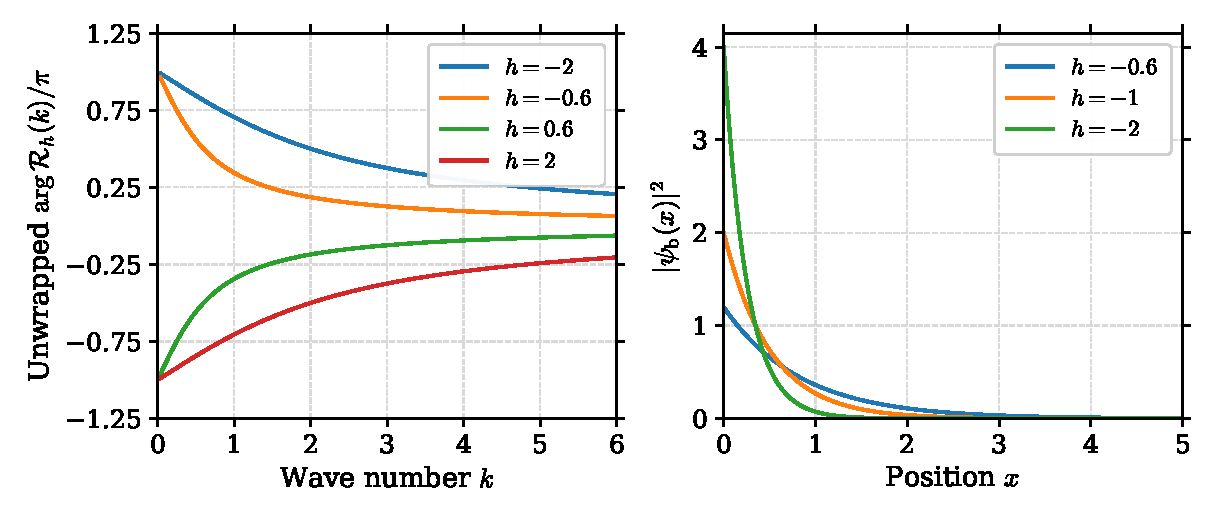
\includegraphics[width=.84\linewidth]{content/MathSkills/figures/geometry-highspin/robin_scattering.pdf}
\caption{不同自伴边界参数 $h$ 下的精确反射相位及归一化束缚态。左图用 $\arg\mathcal R_h(k)$ 的连续分支表征谱参数对散射的影响；右图仅对 $h<0$ 显示 $|\psi_{\mathrm b}(x)|^2$。两者共享同一个边界参数，没有对连续谱进行人为截断。}
\label{fig:ghs-r7-robin-scattering}
\end{figure}

一般度规上的边界不一定是一点，边界 Cauchy 数据可能属于无限维 Sobolev 空间；这时 $h$ 被边界上的自伴算子或 Lagrange 子空间取代，预解差通常也不再是秩一。半直线模型的重要性，在于自伴性、谱测度、负能束缚态及散射矩阵能够在同一套约定下逐式验证，从而为一般的边界谱问题提供最小的完整范例。

二维双曲空间的测地极坐标度规是 $\dd r^2+\sinh^2r\,\dd\theta^2$，故
\[
\Delta_{\mathbb H^2}=\partial_r^2+\coth r\,\partial_r
+\frac{1}{\sinh^2r}\partial_\theta^2.
\]
设 $\phi=R_m(r)\ee^{\ii m\theta}$，则方程 $-\Delta\phi=\lambda\phi$ 变为
\begin{equation}\label{eq:ghs-r6-hyperbolic-radial}
-R_m''-\coth r\,R_m'
+\frac{m^2}{\sinh^2r}R_m=\lambda R_m.
\end{equation}
在 $r\to\infty$ 时，$\coth r=1+O(\ee^{-2r})$ 且角势指数衰减，所以领先径向方程是
$-R''-R'=\lambda R$。令 $R\sim\ee^{sr}$ 后得 $s^2+s+\lambda=0$，根为
\[
s=-\frac12\pm\sqrt{\frac14-\lambda}.
\]
因此当 $\lambda=1/4+\rho^2$、$\rho\in\RR$ 时，远区两支行为是 $\ee^{-r/2\pm\ii\rho r}$。这里 $1/4$ 是连续谱的自然阈值；完整断言 $\operatorname{spec}(-\Delta_{\mathbb H^2})=[1/4,\infty)$ 且无 $L^2$ 点谱，仍需双曲空间调和分析或相应正性估计，不能只凭此渐近 ODE 作全谱证明。

球面角动量只描述角向分解，不能决定散射相位。若背景或势保持旋转对称，每个 $\ell$ 通道的径向自伴算子仍可能含不同的边界参数、束缚态与连续谱相移；相关可观测量要从其解析预解、Jost 解及壳上散射矩阵提取。在一般非球对称背景，各 $\ell$ 通道还会耦合成矩阵值散射问题。此时更普适的对象是完整的谱投影和散射算子，而不是把某一条球面高自旋定则推广成普遍结论。

一维边界问题说明了定义域为什么重要。对真正的标量、矢量或张量场，还需要确定其协变微分算子，之后才能从整个谱构造热核与 Green 函数。

\subsection{区间逆核的直接计算}
\label{app:ghs-spectral-tests}



对区间 $(0,L)$ 上的算子 $A=-\frac{\dd^2}{\dd x^2}+m^2$，$m>0$，取 Dirichlet 边界条件。对于固定源点 $y$，齐次方程的两侧解分别可取 $\sinh(mx)$ 与 $\sinh(m(L-x))$。要求 $G(x,y)$ 连续，且
$-\partial_xG(y^+,y)+\partial_xG(y^-,y)=1$，由此唯一得到
\begin{equation}\label{eq:ghs-dirichlet-green-interval}
 G_D(x,y)=\frac{\sinh(m x_<)\sinh[m(L-x_>)]}{m\sinh(mL)},
 \qquad x_<=\min(x,y),\quad x_>=\max(x,y).
\end{equation}
将 $G_D$ 对 $x$ 积分两次，可检查其是 $A^{-1}$ 的积分核。若将边界换成 Neumann，核的边界导数条件改变，零质量极限还要移除常数零模。这一完整计算说明 Green 函数的选择确实依赖算子定义域。

